\documentclass[tikz,margin=0.5mm]{standalone}

% for i in {1..2}; do pdftocairo -f $i -l $i -singlefile -transp -r 350 -png jigsaw.pdf jigsaw$i; done

\usepackage{amsmath}
\usepackage{amssymb}
\usepackage{physics} % \usepackage[arrowdel]{physics}
\usepackage{txfonts} % times for math (for consistency)
\usepackage{times}
\usepackage{jigsaw}

\usepackage{pgfplots}
\usetikzlibrary{calc}
\usetikzlibrary{patterns}
\usetikzlibrary{shapes}
\usetikzlibrary{backgrounds}
\usetikzlibrary{decorations.pathmorphing}
\usetikzlibrary{decorations.markings}

\definecolor{bgcolor}{HTML}{f7f6ee} % grayish

\tikzset{
	every picture/.style={line cap=rect,line width=0.6pt},
	title/.style={black, font=\fontsize{5.7pt}{5.7pt}\selectfont, inner xsep=0.25em},
	content/.style={black, font=\fontsize{6.7pt}{6.7pt}\selectfont},
}

\gdef\asp{0.85}
\gdef\scale{2.0}

\gdef\sigb{\vb*{\sigma}}
\gdef\taub{\vb*{\tau}}
\gdef\epsb{\dot{\vb*{\epsilon}}}
\gdef\eps#1{\dot{\epsilon}_{#1}}
\gdef\sb{\vb{s}}
\gdef\Eij{E_{ij}}
\gdef\mb{\vb{m}}
\gdef\Dv#1{\dfrac{\mathrm{D} #1}{\mathrm{D}t}\hspace{-0.15em}}

\definecolor{cFL}{RGB}{198,219,239} % flow law 
\definecolor{cMB}{RGB}{218,218,235} % momentum balance
\definecolor{cFM}{RGB}{199,233,192} % fabric model
\definecolor{cVA}{RGB}{253,208,162} % viscous anisotropy
\definecolor{mydarkgray}{RGB}{200,200,200} 
\definecolor{mygray}{RGB}{240,240,240} 

\newcommand{\blockMB}[3]{
\begin{scope}[xshift=1cm,yshift=1cm]
    \piece[#1]{-1}{0}{0}{1}
    \node[content] at (0.630, 0.53) {$-\div\sigb=\rho\vb{g}$};
    \node[content] at (0.630, 0.37) {$\sigb=\taub-p\vb{I}$};
    \node[title, anchor=east] (MB) at (1, 0.9) {Momentum balance};
\end{scope}}

\newcommand{\blockFM}[3]{
\begin{scope}[xshift=1cm,yshift=0cm]
    \piece[#1]{0}{0}{1}{-1}
	\node[content] at (0.5, 0.45) {#3};
    \node[title, anchor=east] (FM) at (1, 0.1) {#2};
\end{scope}}

\newcommand{\blockVA}[3]{
\begin{scope}[xshift=0cm,yshift=0cm]
    \piece[#1]{0}{1}{-1}{0}
	\node[content, align=left] at (0.38, 0.51) {#3};
	\node[title, anchor=west] (VA) at (0, 0.1) {#2};
\end{scope}}

\newcommand{\blockFL}[3]{
\begin{scope}[xshift=0cm,yshift=1cm]
    \piece[#1]{1}{-1}{0}{0}
    \node[content] at (0.5, 0.55) {#3};
    \node[title, anchor=west] (FL) at (0, 0.9) {#2};
\end{scope}}

\begin{document}

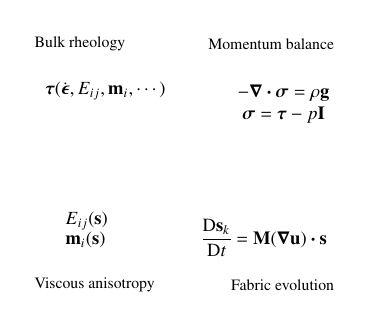
\begin{tikzpicture}[xscale=\scale,yscale={\scale*\asp}]
\blockMB{cMB}{Momentum balance}{}
\blockFM{cFM}{Fabric evolution}{$\Dv{\sb_k}=\vb{M}(\grad\vb{u})\dotproduct\sb$}
\blockVA{cVA}{Viscous anisotropy}{$\Eij(\sb)$\\[0.1em] $\mb_i(\sb)$}
\blockFL{cFL}{Bulk rheology}{$\taub(\epsb,\Eij,\mb_i,\cdots)$}
\end{tikzpicture}

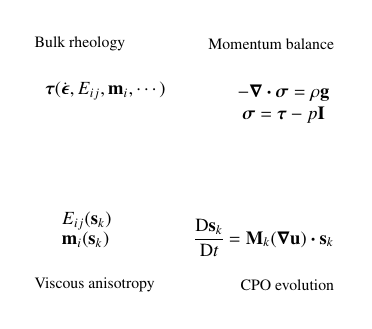
\begin{tikzpicture}[xscale=\scale,yscale={\scale*\asp}]
\blockMB{cMB}{Momentum balance}{}
\blockFM{cFM}{CPO evolution}{$\Dv{\sb_k}=\vb{M}_k(\grad\vb{u})\dotproduct\sb_k$}
\blockVA{cVA}{Viscous anisotropy}{$\Eij(\sb_k)$\\[0.1em] $\mb_i(\sb_k)$}
\blockFL{cFL}{Bulk rheology}{$\taub(\epsb,\Eij,\mb_i,\cdots)$}
\end{tikzpicture}

\end{document}